\section{Nine copper coins, and other toposes}\label{sec_coins}
\epigraph{
	Explicaron que una cosa es \emph{igualdad}, y otra \emph{identidad}, y formularon una especie de \emph{reductio ad absurdum}, o sea el caso hipotético de nueve hombres que en nueve sucesivas noches padecen un vivo dolor. ¿No sería ridículo -interrogaron- pretender que ese dolor es el mismo?
}{JLB ---Tl\"on, Uqbar, Orbis Tertius}

According to our description of the Mitchell-Bénabou language in the category of variable sets, \emph{propositions} are morphisms of the form
\[p : U \to \Omega_I\]

where $\Omega_I$ is the subobject classifier of $\Set/I$ described in \autoref{variable_sets_have_omega}; now, recall that
\begin{itemize}
	\item the object $\Omega_I = \{0,1\}\times I \to I$ becomes an object of $\Set/I$ when endowed with the projection $\pi_I : \Omega_I \to I$ on the second factor of its domain;
	\item the universal monic $\tr : I \to \Omega_I$ consists of a section of $\pi_I$, precisely the one that sends $i : I$ to the pair $(i,1) : \Omega_I$;
	\item every subobject $U \hookrightarrow A$ of an object $A$ results as a pullback (in $\Set/I$) along $\tr$:
	      \[\xymatrix@R=5mm@C=5mm{
		      U\ar[dr]^u\ar[rr]^u\ar[dd]_m&& I\ar[dd]^{\tr} \ar@{=}[dl]\\
		      &I& \\
		      A \ar[ur]\ar[rr]_{\chi_U}&& \ar[ul]\Omega_I
		      }\]
	      (see \autoref{variable_sets_have_omega} for a complete proof)
\end{itemize}
The set $I$ in this context acts as a \emph{multiplier} of truth values, in that every proposition can have a pair $(\epsilon, i)$ as truth value. We introduce the following notation: a proposition $p : U \to \Omega_I$ is \emph{true}, in context $x :U$, with \emph{strength} $t$, if $p(x) =(1,t)$ (resp., $p(x)=(0,t)$).
\begin{remark}\label{very_importanta_force}
	A proposition in the internal language of variable sets is a morphism of the following kind: a function $p : U \to \Omega_I$, defined on a certain domain, and such that
	\[
		\xymatrix{
			U\ar[d]_u\ar[r]^-p  & \{0,1\}\times I \ar[d]^{\pi_I}\\
			I \ar@{=}[r]& I
		}
	\]
	(it must be a morphism of variable sets!) This means that $\pi p(x : U) = u(x : U)$, so that $p(x) = (\epsilon_x, u(x))$ for $\epsilon_x =0,1$ and $u$ is uniquely determined by the "variable domain" $U$. This is an important observation: the strength with which $p$ is true/false is completely determined by the structure of its domain, in the form of the function $u : U \to I$ that renders the pair $(U,u)$ an object of $\Set/I$.
\end{remark}
To get a grip of the different roles of various classes of propositions, and given that our interest will be limited to a certain class of particular propositions that we will construct \emph{ex nihilo}, it is now convenient to discuss what constraints we have to put on the structure of $I$: of course, the richest this structure is, the better will the category $\Set/I$ behave: it is for example possible to equip $I$ with an order structure, or a natural topology. Among different choices of truth multiplier, yielding different categories of variable sets, and different kinds of internal logic therein, we will privilege those that make $I$ behave like a space of strengths: a dense, linear order with LUP, thus not really far from being a closed, bounded subset of the real line.

The main result of the present section is a roundup of examples showing that it is possible to concoct categories of variable sets where some seemingly paradoxical constructions coming from J.L. Borges' literary world have, instead, a perfectly ``classical'' behaviour when looked with the lenses of the logic of variable set theory.

Each of the examples in our roundup \autoref{bla} \autoref{bli} \autoref{blu} is organised as follows: we recall the shape of a paradoxical statement in Borges' literary world. Then, we show in which topos this reduces to an intuitive statement expressed in the syntax of a variable set category.

More than often, we use $I=[0,1]$ as base of variable sets; as already said, there are different reasons for this choice: the most intuitive is that if a truth value is given with a \emph{strength} $t\in I$ it is a natural request to be able to \emph{compare} elements in this set; in particular, it should always be possible to assess what truth value is stronger.

For this reason, even if this assumption is never strictly necessary (the only constraint is that $I$ is totally, or partially, ordered set by a relation $\le$), a natural choice for $I$ is a \emph{continuum} (=a dense total order with LUP --see \cite{moschovakis2009descriptive}). An alternative choice drops the density assumption: in that case the (unique) finite total order $\Delta[n] = \{0 < 1 <\dots < n\}$, or the countable total order $I=\omega = \bigcup_n \Delta[n]$ are all pretty natural choices for $I$ (although it is way more natural for $I$ to have a minimum \emph{and} a maximum element).\footnote{We're only interested in the notion of an abstract interval here: a continuum $X$ endowed with an operation $X \to X \vee X$ of ``zooming'', uniquely defined by this property. In a famous paper Freyd characterises ``the interval'' as the terminal interval coalgebra: see \cite[§1]{freyd2008algebraic}; for our purposes, note that $[0,1]$ is a natural choice: it is a frame, thus a Heyting algebra $\fkH =([0,1],\land,\lor,\Rightarrow)$ with respect to the pseudo-complement operation given by $(x \Rightarrow z) := \bigvee_{x\land y \le z} y$ (it is immediate that $x \land a \le b$ if and only if $a \le x \Rightarrow b$ for every $a,b\in [0,1]$).} In each of these cases ``classical'' logic is recovered as a projection: propositions $p$ can be true or false with strength $1$,\footnote{Here $I$ is represented as an interval whose minimal and maximal element are respectively $0$ and $1$; of course these are just placeholders, but it is harmless for the reader to visualise $I$ as the interval $[0,1]$.} the maximum element of $I$:
\begin{center}
	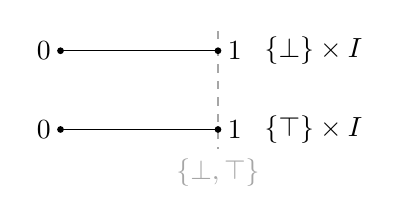
\begin{tikzpicture}
		\draw[gray!70,dashed] (2,1.25) -- (2,-.25) node[below] {$\{\perp,\top\}$};
		\draw[fill] (0,0) circle (1pt) node[left] {$0$};
		\draw[fill] (2,0) circle (1pt) node[right] (dis) {$1$};
		\draw (0,0) -- (2,0);
		\begin{scope}[yshift=1cm]
			\draw[fill] (0,0) circle (1pt) node[left] {$0$};
			\draw[fill] (2,0) circle (1pt) node[right] (dat) {$1$};
			\draw (0,0) -- (2,0);
			\node[right of=dis] {$\{\top\}\times I$};
			\node[right of=dat] {$\{\perp\}\times I$};
		\end{scope}
	\end{tikzpicture}
\end{center}
In order to aid the reader understand the explicit way in which $I$ ``multiplies'' truth values, we spell out explicitly the structure of the subobject classifier in $\Set/\Delta[2]$. In order to keep calling the minimum and maximum of $I$ respectively $0$ and $1$ we call $\frac{1}{2}$ the intermediate point of $\Delta[2]$.
\begin{remark}
	The subobject classifier of $\Set/\Delta[2]$ consists of the partially ordered set $\Delta[1]\times\Delta[2]$ that we can represent pictorially as a rectangle
	\[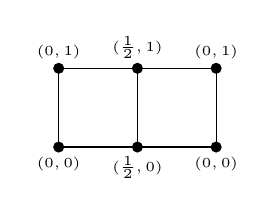
\begin{tikzpicture}[xscale=2]
			\foreach \i/\name in {0/0,.5/{\frac{1}{2}},1/0}{
			\foreach \j/\pos in {0/below,1/above}
			\fill (\i,\j) ellipse (1pt and 2pt) node[\pos] {\tiny $(\name,\j)$};
			}
			\draw (0,0) rectangle (1,1);
			\draw (.5,1) -- (.5,0);
		\end{tikzpicture}\]
	endowed with the product order. The resulting poset is partially ordered, and in fact a Heyting algebra, because it results as the product of two Heyting algebras: the Boole algebra $\{0<1\}$ and the frame of open subsets of the Sierpinski space $\{a,b\}$ (the topology is $\tau_S = \{\varnothing, \{a\}, \{a,b\}\}$).
\end{remark}
\begin{remark}\label{alcuni_set}
	Siccome il caso $I=[0,1]$ con la topologia euclidea è quello piu naturale per diversi motivi, definiamo alcuni insiemi di interesse per una data proposizione $p : U \to \Omega_I$ per questa scelta di $I$:
	\begin{itemize}
		\item $A^\top = \{x : U \mid p(x) = (1,t_x), t_x > 0\} = p^\leftarrow(\{1\}\times (0,1])$ e $A^\perp = \{x : U \mid p(x) = (0,t_x), t_x > 0\}$; cose vere (risp., false) con forza maggiore di zero. Sono le funzioni $u : U \to I$ tali che $u^\leftarrow 0 = \varnothing$.
		\item $B^\top = \{x : U \mid p(x) = (1,1)\} = p^\leftarrow((1,1))$ \footnote{Si può interpretare anche come \emph{"le cose persistono nel tempo"}, e abbiamo catturato la nozione di time-persistence, cfr. 1.4} e $B^\perp = \{x : U \mid p(x) = (0,1)\}$ cose vere (risp.,false).
		\item $E_t^\top = \{ x : U \mid p(x)=(1,t)\}$ e $E_t^\perp = \{ x : U \mid p(x)=(0,t)\}$; cose vere (risp., false) con forza $t$.
	\end{itemize}
\end{remark}
Last but not least, a crucial assumption will be that the strength of $p$ depends continuously, or not, on the variables on its domain of definition. Without such continuous dependence, small changes in context $x : U$ might drastically change the truth value $p(x)$.\footnote{There is no a priori reason to maintain that $p$ is a continuous proposition; one might argue that discontinuous changes in truth value of $p$ happen all the time in ``real life''; see the family of paradoxes based on so-called \emph{separating instants}: how well-defined the notion of ``time of death'' is? How well-defined the notion of ``instant in time''?}
\subsection{The unimaginable topos theory hidden in Borges' library}
Jorge Luis Borges' literary work is well-known for being made by paradoxical worlds; oftentimes, seemingly absurd consequences follow by stretching to their limit ideas from logic and mathematics: time, infinite, self-referentiality, duplication, recursion, the relativity of time, the illusory nature of our perceptions, the limits of language, its capacity to generate worlds.

In the present section we choose \emph{Fictions}, Borges' famous collection of novels, as source of inspiration for possible and impossible worlds and their ontology.

Usualmente la costruzione di un ``mondo impossibile'' (variamente impiegato nelle semantiche paraconsistenti) va circa come segue: since the classic work of Rescher and Brandom [\cite{??}] it is obtained with recursive operations on (kripkean) standard worlds \dots ; noi rovesciamo tale prospettiva, e invece di depennare dal computo degli universi i mondi le cui caratteristiche do not comply with sensorial experience, or imply paradoxical entities/constructs, we accept their existence for bizarre that it may seem, and we try to deduce what kind of logic can consistently generate such statements.

The interest in such a literary calembour is manifold, and the results are surprising:
\begin{itemize}
	\item we unravel how a mathematically deep universe Borges has inadvertently created: of the many compromises we had to take in order to reconcile literature and the uniderlying mathematics,\footnote{See \autoref{our_beloved_interval} below: these ``compromises'' mainly amount to assumptions on the behaviour of space-time on Tl\"on and Babylon.} we believe no one is particularly far-fetched one;
	\item we unravel how \emph{relative} ontological assumptions are; they are not given: using category theory, ontology, far from being the presupposition on which it is based, is a byproduct of language itself. The more expressive language is, the more ontology; the fuzzier its capacity to assert truth, the fuzzier existence becomes;
	\item ``Fuzziness'' of existence, i.e. the fact \emph{entia} exist less than completely, is hard-coded in the language (in the sense of \autoref{da_lang}) of the category we decide to work in from time to time;
	\item ...
\end{itemize}
To sum up, readers willing to find an original result in this paper, might find it precisely here: we underline how Borges' alternative worlds (Babylon, Tl\"on \ dots) are mathematically consistent places, worthy of existence as much as our world, just based on a different internal logic. And they are so just thanks to a base-sensitive theory of existence --ontology breaks in a spectrum of ontolog\emph{ies}, one for each category/world.

The first paradox we aim to frame in the right topos is the famous nine copper coins argument, used by the philosophers of Tlön to construct a paradoxical object whose existence persists over time, in absence of a consciousness continually perceiving it and maintaining in a state of being.
\begin{example}[Nine copper coins]\label{bla}
	First, we recall the exact statement of the paradox:\footnote{The paradox appears in a primitive, mostly unchanged version in \cite{borges1997otras}, where instead of nine copper coins, a single arrow, shot by an anonymous archer, disappears among the woods. For what concerns Tl\"on's  nine copper coins, our translation comes from \cite{tlonEN}:
		\begin{quote}
			\hspace{.5em} Tuesday, $X$ crosses a deserted road and loses nine copper coins. On Thursday, $Y$ finds in the road four coins, somewhat rusted by Wednesday's rain. On Friday, $Z$ discovers three coins in the road. On Friday morning, $X$ finds two coins in the corridor of his house. The heresiarch would deduce from this story the reality - i.e., the continuity - of the nine coins which were recovered.

			\hspace{.5em} It is absurd (he affirmed) to imagine that four of the coins have not existed between Tuesday and Thursday, three between Tuesday and Friday afternoon, two between Tuesday and Friday morning. It is logical to think that they have existed - at least in some secret way, hidden from the comprehension of men - at every moment of those three periods.
		\end{quote}}
	\begin{quote}
		El martes, $X$ atraviesa un camino desierto y pierde nueve monedas de cobre.
		El jueves, $Y$ encuentra en el camino cuatro monedas, algo herrumbradas por la lluvia del miércoles. El viernes, $Z$ descubre tres monedas en el camino. El viernes de mañana, $X$ encuentra dos monedas en el corredor de su casa. El  quería deducir de esa historia la realidad -id est la continuidad- de las nueve monedas recuperadas.

		Es absurdo (afirmaba) imaginar que cuatro de las monedas no han existido entre el martes y el jueves, tres entre el martes y la tarde del viernes, dos entre el martes y la madrugada del viernes. Es lógico pensar que han existido -siquiera de algún modo secreto, de comprensión vedada a los hombres- en todos los momentos de esos tres plazos.
	\end{quote}
	Before going on with our analysis, it is important to remark that there is one and only one reason why the paradox of the nine copper coins is invalid: copper does not rust. Incidentally, we will be able to propose a rectification of this ``rust counterargument'' without appealing to the assumption that copper can rust on Tl\"on due to a purported difference between Earth's and Tl\"onian chemistry.

	It is obvious on what this construction leverages to build an efficient aporia: the unimaginable persistence of things through time, even without a perceivent consciousness.

	Expressed in natural language, our solution to the paradox goes more or less as follows: $X$ loses their coins on Tuesday, and the force $\varphi$ with which they ``exist'' lowers; it grows back in the following days, going back to a maximum value when $X$ retrieves two of their coins on the front door. $Y$ findings of other coins raises their existence force to a maximum. The coins that $Y$ has found rusted (or rather, the surface copper oxidized: this is possible, but water is rarely sufficient to ignite the process alone --certainly not in the space of a few hours.
	% \footnote{in una sorta di principio di wormhole, eventi indipendenti sulla terra sono dipendenti su Tlön, perché l'evento A influenza, in uno spazio pluridimensionale di scelte di z di verità, l'evento B in modi che gli sarebbero vietati se fosse sulla Terra.}
	\begin{remark}\label{our_beloved_interval}
		In this perspective, Tl\"on classifier of truth values can be taken as $\Omega_I = \{0<1\}\times I$, where $I$ is any set with more than one element; a minimal example can be $I=\{N,S\}$ (justifying this choice from inside Tl\"on is easy: the planet is subdivided into two emispheres; each of which now has its own logic ``line'' independent from the other), but as explained in \autoref{our_beloved_interval} a more natural choice for our purposes is the closed real interval $I=[0,1]$.

		This allows for a continuum of possible forces with which a truth value can be true or false;  it is tobe noted that $[0,1]$ is also the most natural place on which to interpret fuzzy logic, albeit the interest for $[0,1]$ therein can be easily and better motivated starting from probability theory. (There are interesting perspective on how to develop basic measure theory out of $[0,1]$. For example, measures valued in things like Banach space and more general topological	vector spaces have been considered.)
	\end{remark}
	We now start to formalise properly what we said until now. To set our basic assumptions straight, we proceed as follows:
	\begin{itemize}
		\item Without loss of generality, we can assume the set $C = \{c_1,\dots,c_9\}$ of the nine coins to be totally orered and partitioned in such a way that the first two coins are those retrieved by $X$ on Tuesday, the subsequent four are those found by $Y$ on their way, and the other three are those seen by$Z$. So,
		      \[C = C_X \sqcup C_Y \sqcup C_Z.\]
		      and $C_X = \{c_{X1}, c_{X2}\}$, $C_Y = \{c_{Y1},c_{Y2},c_{Y3},c_{Y4}\}$, $C_Z= \{c_{Z1}, c_{Z2}, c_{Z3}\}$ As already said, the truth multiplier $I$ is the closed interval $[0,1]$ with its canonical order --so with its canonical structure of Heyting algebra, and if needed, endowed with the usual topology inherited by the real line.
		\item Propositions of interest for us are of the following form:
		      \[\lambda gcd.p(g, c, d) : \{X,Y,Z\}\times C\times W \to \Omega_I\]
		      where $W \subseteq \{\S,\M,\Tu,\W, \Th,\F,\Sa\}$ is a set of days (strictly speaking, the paradox involves just the interval $[\Tu,\F]$). The value $p(g,c,d)$ models how in $g$'s frame of existence the coin $c$ exists at day $d$ with strength $p(g,c,d)$.
	\end{itemize}
	\begin{definition}[Admissible coins]
		We now define an \emph{admissible} configuration of coins any arrangement of $C$ such that the following two conditions are satisfied:
		\begin{enumtag}{ad}
			\item for all day $d$ and coin $c$, we have
			\[
				\sum_{u\in \{X,Y,Z\}} p(u,c,d) = (\top, 1)
			\]
			where we denote as ``sum'' the logical conjunction in $\Omega_I$: this means that day by day, the \emph{global} existence of the group of coins constantly attains the maximum; it is the \emph{local} existence that lowers when the initial conglomerate of coins is partitioned.
			\item Moreover,
			\[
				\begin{cases}
					\sum_{c_X\in C_X} p(X,c_X,V) = (\top,1) \\
					\sum_{c_Y\in C_Y} p(Y,c_Y,G) = (\top,1) \\
					\sum_{c_Z\in C_Z} p(Z,c_Z,V) = (\top,1)
				\end{cases}
			\]
		\end{enumtag}
	\end{definition}
	In an admissible configuration the subsets $ C_X, C_Y, C_Z $ can only attain an existence $p(g,c,d) \lneq (\top,1)$; that is to say, \emph{no coin completely exists locally}. But for an hypothetical external observer, capable of observing the system, adding up the forces with which the various parts of $C$ exist, the coins \emph{globally} exist `` in some secret way, of understanding forbidden to men'' (or rather, to $ X, Y, Z $).
	\begin{center}
		\begin{figure}[h]
			\begin{tikzpicture}[xscale=6, yscale=4]
				\coordinate (1) at (0,0);
				\foreach \i/\j in {1/\W,2/\Th,3/\F}{
						\draw[gray!90] (\i/4,0) node[below] {\tiny \j} -- (\i/4,1);
					}
				\node[below,gray!90] at (0,0) {\Tu};
				\node[below,gray!90] at (1,0) {\Sa};
				\coordinate (1) at (0,0);
				\coordinate (2) at (1/2, 1/5);
				\coordinate (3) at (3/4,1);
				\draw[ultra thick,red] (1) -- (2) node[right] {\scriptsize $1/5$} -- (3);
				\draw[thin,yellow] (1) -- (2) -- (3);
				\draw[blue] (1) -- (1/2,1) node[above] {\scriptsize $p(Y, c_Y)=(\top,1)$} -- (3/4,1/4) node[right] {\scriptsize $1/4$};
				\node[fill=gray!60] (cloud) at (1/4,1/2) {\large\color{black} \faCloud};
				\draw[thick] (0,0) rectangle (1,1);
			\end{tikzpicture}
			\caption{A pictorial representation of the truth forces of coins in different days; we choose a minimally complex, piecewise linear model where strength of existence goes up and down linearly to join the points where \cite{tlonEN} gives complete information about the coins' configuration. $X$ is marked in red, $Z$ in yellow, $Y$ in blue. Time is considered as a continuum line, marked at weekdays for readability.}
			\label{fig_coins}
		\end{figure}
	\end{center}
\end{example}
\begin{remark}
	An important claim is now in order, as our construction might appear just a sleight of hand leaving open the main problem posed by the coin riddle: \emph{where} do the coins exist? Not to mention that to some extent, \emph{every} theory of existence posits that things are there in some secret way. Tl\"on's idealist might deny time (our model makes no strong assumption on what time is made of: discrete, continuous, homogeneous, slowed by traveling at high speed\dots); $B^\bot$ ontologists live comfortably in $B^\bot$, as defined in \autoref{alcuni_set} without being able to tell anything about how objects ``completely do not exist''.
	At the opposite side of the spectrum the pure empiricist lives in $B^\top$, and they're unable to tell how they ``completely exist'').

	This is where our analysis comes in handy; in particular, this is where our particular choice of $\Omega_I$ plays its r\^ole. In our model $B^\perp, B^\top$ are just particular slices of a single object where they coexist as particular fibers; the approach that looks at them as such is \emph{inherently better}, as it yields a quantitative answer framing both $B^\top$- and $B^\bot$-ontology as opposite sides of a spectrum made out of diverse colours.
\end{remark}
\begin{example}
	An example of an admissible configuration of coins is the following (cf. \autoref{fig_coins}): we assume strength of existence goes up and down linearly to join the points where we have information about total existence of the subsets $C_X,C_Y,C_Z$: in the remaining instants of time, the coins out of sight for $X$ share an equal amount of existence in such a way that constraints \ref{ad:uno} and \ref{ad:due} above are satisfied: in this particular example, $p(Y,c_Y,\Th) = (\top,1)$, whereas $p(X,C_X,\Th)=p(Z,C_Z,\Th)=(\top,1/5)$, and $p(Y,c_Y,\F)=(\top,1/4)$, whereas $p(X,C_X,\F)=p(Z,C_Z,\F)=(\top,1)$.
\end{example}
\begin{italian}
	\begin{remark}\label{di_navi_e_numeri}
		L'aritmetica di Tlon; proposizioni a forza additiva; parallelismi tra la nave di Teseo e le nove monete.
	\end{remark}
\end{italian}
\begin{remark}[Continuity for a proposition]\label{continuiti}
	Let $p : U \to \Omega_I$ be a proposition; here we investigate what does it mean for $p$ to be (globally) continuous with respect to the Euclidean topology on $I=[0,1]$, in the assumption that its domain of definition $U$ is metrisable (this is true for example when $U$ is a subset of space-time). The condition is that
	\[ \forall \epsilon > 0,\,\exists \delta > 0 : |x-y|< \delta \To |px-py| < \epsilon \]
	Da questo segue immediatamente che quando $p$ è continua nel suo dominio, i valori di verità di $p$ in configurazioni ``vicine'' in un senso opportuno sono dati con forze allo stesso modo vicine (chiaramente questa è una descrizione spannometrica della nozione di continuità\dots).

	All elementary topology results apply to such a proposition: for example the set of forces with which $p$ is true or false is a connected subset of $\Omega_I$, compact if $U$ was compact.
\end{remark}
Continuity and discontinuity of a proposition $p : U \to \Omega_I$ now capture quite well other pieces of Borges' literary universe: here we provide two examples. We refrain from a deep, quantitative analysis, and we invite the reader to fill the details of our reasoning as a pleasant re-reading exercise of \cite{babil} and \cite{tlonEN}.\footnote{The plot of \cite{babil} in a nutshell is: in Babylon, a lottery game infiltrates reality to the point that it ends up governing the actions of all men; freeing them from free will while coorting them into pawns of an infinite, inescapable, unknowable game, governed by an iron, seemingly chaotic, probabilistic logic.}
\begin{example}[Discontinuity, sapphire from Taprobana]\label{bli}
	Propositions $p : U \to \Omega_{[0,1]}$ that are allowed to be discontinuous in its variables depend unpredictably from their context: such propositions model seemingly chaotic events triggered as the end terms of a chain of disconnected prior events; in fact, if we assume a real base for the domain of $p$, its continuity as stated in \autoref{continuiti} roughly means that events in the same neighbourhood --``near'' in space or temporally contiguous-- can't have too much different truth/force values.

	A model for such a universe, where ``terrible consequences'' sometimes follow from the ``impersonal drawings, whose purpose is unclear'' characterising the Company's actions: seemingly disconnected (that ``a sapphire from Taprobana be thrown into the waters of the Euphrates''; that ``a bird be released from the top of a certain tower''; that ``every hundred years a grain of sand be added to (or taken from) the countless grains of sand on a certain beach''), but generating nontrivial dynamics when inserted in a suitable sequence as in \autoref{fig_dynamics}.

	Let us consider the dynamical system $(\nabla\circ p, [0,1])$ obtained from the iterates of the composition $\nabla \circ p : [0,1] \to [0,1]$ ($\nabla : I\amalg I \to I$ is the fold map of $I$, obtained from the identity of $I$ and the universal property of the coproduct). We start from a proposition $p$ depending on a free variable $t : I$; then, $p(t) = (u(t),\epsilon)\in \Omega_I$ consists of a force and a truth value; but $p$ can be evaluated on $u(t)$ (although this is not its universal property, the fold map $\nabla$ just forgets the truth value, keeping the force): the process can thus be iterated as follows, exploiting the universal property of the natural number object in $\Set/I$:
	\begin{center}
		\begin{figure}[h]
			\def\line{\draw (0,0) -- (1,0); \draw (0,.5) -- (1,.5);}
			\begin{tikzpicture}
				\line
				\fill (.395,0) circle (1pt);
				\foreach \i/\j/\k in {2.25/.382/0,4.5/.537/.5,6.75/.874/.5,9/.128/0}{
						\begin{scope}[xshift=\i cm]
							\line
							\fill (\j,\k) circle (1pt);
							\node at (-.5,.375) {$\overset{\scriptscriptstyle\nabla\circ p}\mapsto$};
						\end{scope}
					}
			\end{tikzpicture}
			\caption{A dynamical system induced by the Company's infinite, impersonal drawings.}
			\label{fig_dynamics}
		\end{figure}
	\end{center}
	It is clear that the limit behaviour of such a sequence strongly depends on the analytic properties of $f$ (cf. \cite{strogatz1996nonlinear} for an intro to one-dimensional dynamic systems and for their applications see \cite{wiggins2003introduction}). In a well-known procedure, a repeated series of drawings can chaotically deform the configuration space on which $p$ is evaluated.\footnote{There is of course countless termination conditions on such process $p$; the series can be periodic, it can stop when $p$ reaches maximum or minimum force, or a prescribed value, or is inside/outside a certain range of forces\dots; we leave such speculations to the mystagogues of the Company, or to the lions of Qaphqa.}
\end{example}
Another compelling example is that of the monotonicity of a proposition depending, say, on a certain number of observers who acknowledge the ``existence'' of an object $R$ (be it physical or conceptual) in large numbers, from which very reason the existence of $R$ gains strength.
\begin{example}[Continuity: a few birds, a horse]\label{blu}
	Let us consider objects whose existence strength depends \emph{monotonously} and continuously from their parameters: for example a proposition $p$ may be ``truer'' the more people observe it, because
	\begin{quote}
		things became duplicated in Tlön; they also tend to become effaced and lose their details when they are forgotten. A classic example is the doorway which survived so long it was visited by a beggar and disappeared at his death. At times some birds, a horse, have saved the ruins of an amphitheater.  \hfill\cite{tlonEN}
	\end{quote}
	In such a situation, we can note that the strength of existence of some ruins --modeled as it is the more naive to do, like a rigid body $R$ in space-- depends on the number of its observers:
	\[\textstyle p(R, n) = \big(\top, 1-\frac{1}{n}\big)\]
	\begin{figure}[h]
		\begin{center}
			\begin{tikzpicture}[xscale=1.25]
				\draw[->, thick, >=stealth] (0,0) -- (6,0);
				\foreach \j/\i in { 1/.2
						, 2/.35
						, 3/.55
						, 4/.8
						, 5/1
					}
				\node[opacity=\i] at (\j,.65) {\fontsize{30}{30}\selectfont \Tribar};
			\end{tikzpicture}
		\end{center}
		\caption{On Tl\"on, there are things that exist stronger the more you believe in them. This is a consequence of the strength $p(\Tribar)$ monotonically depending on an increasing variable $n$ (``trust'' in that existence, ``belief'' that the impossible tribar \Tribar exists.)}
	\end{figure}
\end{example}
A last, somewhat dramatic example. What happens if we change topology on $I$? For example, we could brutally forget the Euclidean topology of the closed interval $[0,1]$, and regard $I$ as the disjoint union $\{ \{t\} \mid t\in [0,1]\}$ of its points; so, the subobject classifier becomes the disjoint union of $[0,1]$ copies of $\{\perp,\top\}$. (See \autoref{fig:berkeley} below for a picture.)
\begin{example}[La campagna incendiata]\label{incendiata}
	Il Berkeley idealista degli infiniti istanti di tempo continuo, disconnessi e incomunicabili: $\Omega_I = \coprod_{t : [0,1]} \{ \perp,\top\}$. Questa particolare struttura logica influences language making it become berkeleyan \emph{instantaneism}: terms of the perceptual bundle are recorded and stockpiled by instantaneous accretion, by disjoint sum of their constituents: ``round airy-light on dark'' or ``pale-orange-of-the-sky''; objects are determined by their simultaneity, instead of their logical dependence: accretion builds meaning, temporal sequentiality is just an illusion, a mistake of perception.
	\begin{quote}
		\hspace{.5em} Spinoza ascribes to his inexhaustible divinity the attributes of extension and thought; no one in Tlön would understand the juxtaposition of the first (which is typical only of certain states) and the second - which is a perfect synonym of the cosmos. In other words, they do not conceive that the spatial persists in time. The perception of a cloud of smoke on the horizon and then of the burning field and then of the half-extinguished cigarette that produced the blaze is considered an example of association of ideas.   \hfill\cite{tlonEN}
	\end{quote}
	(Berkeleyan instantaneism is, of course, way larger than a paragraph: we explore the consequences of this principle in \autoref{di_navi_e_numeri}, in form of a link between Berkeley, the additive nature of truth force in Tl\"on, and its peculiar arithmetic.)
	\begin{center}
		\begin{figure}[h]
			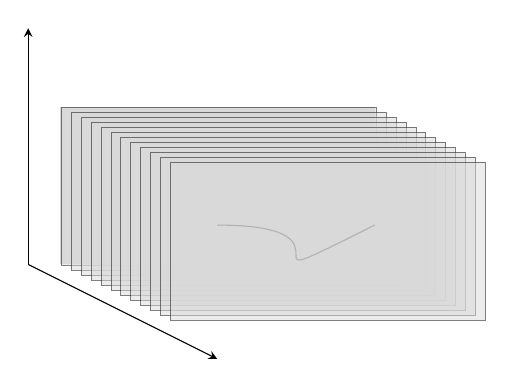
\begin{tikzpicture}[xscale=4, yscale=2]
				\fill[gray!30] (0,0) rectangle (1,1);
				\foreach \i in {.1,1,...,10}
				\draw[xshift=\i, yshift=-\i, ultra thin, fill=gray!30, opacity=.5] (0,0) rectangle (1,1);
				\draw[->, >=stealth, thin] (-.1,0) -- (-.1,1.5);
				\draw[->, >=stealth, thin] (-.1,0) -- (.5,-3/5);
				\draw[gray!60, xshift=.5cm, yshift=.25cm] (0,0) .. controls (.5,0) and (0,-.5) .. (.5,0);
			\end{tikzpicture}
			\caption{Times as an infinite, and infinitely subdivided, sequence of distinguished instants: the ``Berkeley paradox'' of non existence of causality lives in a topos, as nearby slices $E_t, E_s$ for small $|s-t|$ give no predictive power on how (and if) the transition from $E_t$ to $E_s$ might happen.}
			\label{fig:berkeley}
		\end{figure}
	\end{center}
\end{example}